\documentclass[12pt,a4paper]{article}
\usepackage{fontspec}
\setmainfont{Times New Roman}
\setsansfont{Arial}
\setmonofont{Courier New}
\usepackage[provide=*,english,romanian]{babel}
\usepackage{amsmath,amssymb,graphicx,geometry,setspace}
\usepackage{fancyhdr,caption,float,listings,xcolor,booktabs,longtable,array,calc}
\usepackage{subcaption,etoolbox,upquote}
\usepackage[unicode,hidelinks]{hyperref}
\geometry{top=2cm,bottom=2cm,left=2.5cm,right=2.5cm}
\setstretch{1.5}
\setlength{\parindent}{0pt}
\setlength{\parskip}{5pt}
\makeatletter
\renewcommand\section{\@startsection{section}{1}{0pt}{16pt}{7pt}{\normalfont\Large\bfseries}}
\renewcommand\subsection{\@startsection{subsection}{2}{0pt}{12pt}{5pt}{\normalfont\large\bfseries}}
\renewcommand\subsubsection{\@startsection{subsubsection}{3}{0pt}{9pt}{4pt}{\normalfont\normalsize\bfseries}}
\makeatother
\setcounter{secnumdepth}{-1}
\pagestyle{fancy}
\fancyhf{}
\rfoot{\thepage}
\renewcommand{\headrulewidth}{0pt}
\setlength{\headheight}{15pt}
\captionsetup{font=small,labelfont=bf,skip=6pt,justification=raggedright,singlelinecheck=false}
\captionsetup[figure]{position=above}
\lstset{language=C,basicstyle=\ttfamily\fontsize{9.5}{11.5}\selectfont,
  columns=fullflexible,showstringspaces=false,tabsize=2,numbersep=8pt,
  frame=single,rulecolor=\color{black!35},breaklines=true,keepspaces=true,
  xleftmargin=4pt,xrightmargin=4pt,aboveskip=8pt,belowskip=8pt}
\AtBeginEnvironment{lstlisting}{\singlespacing}
\AtBeginEnvironment{longtable}{\small\singlespacing}
\setlength{\emergencystretch}{3em}
\providecommand{\tightlist}{\setlength{\itemsep}{0pt}\setlength{\parskip}{0pt}}
\providecommand{\passthrough}[1]{#1}
\providecommand{\pandocbounded}[1]{#1}
\hypersetup{pdftitle={Sisteme de operare — Laborator 9 și 10},pdfauthor={Tacu Igor}}
\clubpenalty=10000
\widowpenalty=10000
\displaywidowpenalty=10000
\begin{document}
\begin{titlepage}
\thispagestyle{empty}
\begin{center}
\setstretch{1.18}

\includegraphics[width=0.23\textwidth]{scripts/report-style/utm-logo.png}\\[12pt]
\textbf{MINISTERUL EDUCAȚIEI ȘI CERCETĂRII}\\
\textbf{AL REPUBLICII MOLDOVA}\\[4pt]
\textbf{Universitatea Tehnică a Moldovei}\\
\textbf{Facultatea de Calculatoare, Informatică și Microelectronică}\\
\textbf{Departamentul Inginerie Software și Automatică}\\[36pt]
{\fontsize{22}{26}\selectfont\textbf{Raport}}\\[10pt]
Lucrare de laborator nr. 9 și 10\\[8pt]
\textbf{\large Sisteme de operare}\\[24pt]
\textbf{Tema:} Observarea apelurilor de sistem în Linux și implementarea trace în xv6
\end{center}
\vfill
\begin{flushright}
\setstretch{1.25}
Realizat de:\\
stud. gr. FAF-242, Tacu Igor\\[24pt]
Verificat de:\\
Reițman Patricia
\end{flushright}
\vfill
\begin{center}\textbf{Chișinău – 2026 }\end{center}
\end{titlepage}

\setcounter{page}{1}
\section{Scopul lucrării}\label{scopul-lucrux103rii}

Corelarea operațiilor user cu apelurile de sistem observate și
implementarea unui mecanism de trasare selectivă în kernel-ul xv6.

\section{Sarcina lucrării}\label{sarcina-lucrux103rii}

\begin{itemize}
\tightlist
\item
  Observarea apelurilor lui ls și ale programului syscalls, inclusiv
  scrierile pe stdout.
\item
  Explicarea descriptorilor, a celor șase apeluri pe fișier și a
  numărului de apeluri openat.
\item
  Implementarea trace, reproducerea etapei unknown sys call și
  verificarea patch-ului, măștilor și moștenirii la fork.
\end{itemize}

\section{Considerații teoretice}\label{consideraux21bii-teoretice}

Un apel de sistem folosește o interfață numerotată între user și kernel.
Descriptorul 1 este ieșirea standard a procesului, indiferent de
destinația sa concretă. Trasarea arată numele, argumentele sau
rezultatul apelurilor; o mască de biți selectează apelurile urmărite.
Starea de trasare a procesului trebuie inițializată și transmisă corect
la fork.

\section{Implementare. Rezultate
practice}\label{implementare.-rezultate-practice}

\subsection{What can be checked in this
submission}\label{what-can-be-checked-in-this-submission}

Lab 9 observes calls made by a Linux executable, including the
descriptor used for terminal output. Lab 10 adds an observation facility
inside xv6. The two tasks meet at the system-call boundary, but use
different mechanisms: Linux strace is an external tracing program,
whereas the xv6 handler and dispatcher are modified kernel code.

The source is now in the same {\ttfamily\fontsize{10}{12}\selectfont OS}
repository as this report.
{\ttfamily\fontsize{10}{12}\selectfont Lab9-10/sysc\allowbreak{}alls.c}
is the Linux utility. The full
{\ttfamily\fontsize{10}{12}\selectfont xv6} directory contains
{\ttfamily\fontsize{10}{12}\selectfont user/trace.c}, the assembly-stub
generator, the handler, the syscall number and dispatch entry, the
per-process mask, and inheritance in process creation. A reader does not
need to locate a separate fork to assess the implementation. Upstream
MIT code and the changes made for these labs are distinguished in
{\ttfamily\fontsize{10}{12}\selectfont xv6/PROVENAN\allowbreak{}CE.md}.

The new evidence was collected in the Ubuntu 24.04 x86\_64 server and
from QEMU booting that source tree. Console blocks in this report are
excerpts of real text recordings, not reconstructed SSH screenshots. The
complete Linux traces and xv6 console output are included under
{\ttfamily\fontsize{10}{12}\selectfont Lab9-10/evid\allowbreak{}ence};
the runner scripts are committed alongside them.

\subsection{Lab 9 Finding the output descriptor of
ls}\label{lab-9-finding-the-output-descriptor-of-ls}

I compiled the program in a temporary working directory and traced a
plain {\ttfamily\fontsize{10}{12}\selectfont ls -l} there using
{\ttfamily\fontsize{10}{12}\selectfont strace -o ls.trace -e trace=openat\allowbreak{},read,write,\allowbreak{}close ls -l}.
Sending the trace to its own file keeps strace diagnostics separate from
the command's normal stdout. The recorded output call is:

\par\noindent\begin{minipage}{\linewidth}

\begin{lstlisting}
write(1, "total 20\n-rw-r--r-- 1 root root "..., 111) = 111
\end{lstlisting}

\end{minipage}\par

Descriptor 1 is standard output. The return value equals the requested
byte count in this call, showing that the full buffer was accepted. The
buffer includes the long-format listing rather than a message from
strace. Its total length depends on the current directory and listing
layout, so the byte count is not a portable constant. The implementation
of ls can buffer multiple displayed lines before making one write; one
displayed line should not be assumed to imply one system call.

The trace also contains file operations unrelated to the file the lab
program will create: the dynamic loader and library setup open and read
their own files. This matters when interpreting raw strace output. A
read on descriptor 3 near process startup does not necessarily read
{\ttfamily\fontsize{10}{12}\selectfont note.txt}; identifying the
pathname at open time is needed to attribute later uses of that
descriptor. The complete
{\ttfamily\fontsize{10}{12}\selectfont ls.trace} is retained so these
setup calls can be inspected without reducing the trace to a selected
screenshot.

Counting the selected lines in that recording gives 38 calls: 10 openat,
16 close, 11 read, and 1 write. This is the total for the four traced
families; calls excluded by the filter cannot be counted from this
recording.

\subsection{Lab 9 Six calls on
note.txt}\label{lab-9-six-calls-on-note.txt}

The utility creates or truncates
{\ttfamily\fontsize{10}{12}\selectfont note.txt} with mode 0644, writes
{\ttfamily\fontsize{10}{12}\selectfont hello, kernel} plus a newline,
closes it, reopens it read-only, reads into a 64-byte buffer with space
reserved for the terminator, and closes it again. Both opens are checked
before their descriptors are used. A failed read is checked before
indexing the buffer, so a negative return value cannot become an invalid
array offset. Every close is also checked.

These are the six consecutive file calls captured in the new run:

\par\noindent\begin{minipage}{\linewidth}

\begin{lstlisting}
openat(AT_FDCWD, "note.txt", O_WRONLY|O_CREAT|O_TRUNC, 0644) = 3
write(3, "hello, kernel\n", 14)         = 14
close(3)                                = 0
openat(AT_FDCWD, "note.txt", O_RDONLY)  = 3
read(3, "hello, kernel\n", 63)          = 14
close(3)                                = 0
\end{lstlisting}

\end{minipage}\par

There are thirteen visible characters plus the newline, hence fourteen
bytes. The second read requests at most 63 bytes and receives fourteen.
Adding a null byte at {\ttfamily\fontsize{10}{12}\selectfont buf[n]}
makes the returned bytes suitable for a subsequent string print without
writing beyond the buffer. That terminator is a userspace operation and
does not appear as another file write.

The repeated return value 3 is descriptor reuse, not a second permanent
identity for the file. Descriptors 0, 1, and 2 were already occupied by
standard input, output, and error. Closing the first descriptor made
slot 3 available again, so the next open could choose it. The same
integer could name a completely different open file in another part of
the process. The path, inode, and process-local descriptor are related
concepts but cannot be substituted for one another.

Although the source calls C
{\ttfamily\fontsize{10}{12}\selectfont open}, this libc used the Linux
{\ttfamily\fontsize{10}{12}\selectfont openat} syscall with
{\ttfamily\fontsize{10}{12}\selectfont AT\_FDCWD}. The path is relative
to the current working directory. This is a concrete example of why a C
function's name and the traced syscall name need not be identical: the
library selects the actual interface used to request the kernel
operation.

\subsection{Lab 9 The program also writes to
stdout}\label{lab-9-the-program-also-writes-to-stdout}

The status messages use printf, while file data uses write directly. In
the recorded run the program's stdout was redirected to the evidence
log. The stdio messages were buffered and appeared together in one
eighty-byte write:

\par\noindent\begin{minipage}{\linewidth}

\begin{lstlisting}
write(1, "open returned descriptor 3\nwrite sent 14 bytes\nread got 14 bytes: hello, kernel\n", 80) = 80
\end{lstlisting}

\end{minipage}\par

That explains why the status text can appear late in the syscall trace
even though the corresponding printf statements occur between file
operations in the C source. Buffering changes when bytes are handed to
the kernel. It does not mean the source statements executed in a
different order. This stdout call is distinct from
{\ttfamily\fontsize{10}{12}\selectfont write(3, ...)}, which wrote the
fourteen file-data bytes. Keeping both calls in the report makes the
descriptor distinction directly visible.

\subsection{Lab 9 Counting one kind of
call}\label{lab-9-counting-one-kind-of-call}

The repeated count used
{\ttfamily\fontsize{10}{12}\selectfont strace -c -e trace=openat ls -l}
with stdout redirected to
{\ttfamily\fontsize{10}{12}\selectfont /dev/null}. The observed summary
was:

\par\noindent\begin{minipage}{\linewidth}

\begin{lstlisting}
% time     seconds  usecs/call     calls    errors syscall
------ ----------- ----------- --------- --------- ----------------
100.00    0.000125          12        10           openat
------ ----------- ----------- --------- --------- ----------------
100.00    0.000125          12        10           total
\end{lstlisting}

\end{minipage}\par

This run counted ten openat calls without errors. The earlier remote
Ubuntu run counted 31 calls and 18 failed lookups. Both are observations
of their respective environments: the new run fixes
{\ttfamily\fontsize{10}{12}\selectfont LC\_ALL=C} and uses the C locale,
while the earlier run used a different locale configuration. Failed
locale-candidate opens need not make ls fail. It would be incorrect to
present 31 as the number every ls invocation must make, or to merge a
count from one environment with a trace from another.

The brief lists a counting part without a detailed procedure. The
summary command above makes the chosen method explicit. Its timing
columns measure this particular instrumented execution; they are not a
benchmark comparison, and the single short run does not justify
conclusions about system-call performance.

\subsection{Lab 10 Following number 23 across the
boundary}\label{lab-10-following-number-23-across-the-boundary}

The implementation reserves 23 as
{\ttfamily\fontsize{10}{12}\selectfont SYS\_trace} in
{\ttfamily\fontsize{10}{12}\selectfont kernel/sysca\allowbreak{}ll.h},
after the existing sync call at 22.
{\ttfamily\fontsize{10}{12}\selectfont user/user.h} declares
{\ttfamily\fontsize{10}{12}\selectfont trace(int)}, and
{\ttfamily\fontsize{10}{12}\selectfont user/usys.pl} emits its userspace
assembly wrapper. The wrapper places the syscall number in a7 and
executes ecall; the mask travels as the first argument.
{\ttfamily\fontsize{10}{12}\selectfont user/trace.c} validates that a
command was supplied, calls trace with the parsed mask, then invokes
exec on the command and its remaining arguments.

The kernel counterpart is
{\ttfamily\fontsize{10}{12}\selectfont sys\_trace} in
{\ttfamily\fontsize{10}{12}\selectfont kernel/syspr\allowbreak{}oc.c}.
It retrieves argument zero with argint and saves it in the current
process. Returning zero tells the userspace utility that enabling the
mask succeeded. Adding the handler to the dispatch array and declaring
its prototype makes the number executable rather than merely known to
the header. Without that registration, the intermediate experiment
reported {\ttfamily\fontsize{10}{12}\selectfont unknown sys call 23};
the final tree contains the actual handler and dispatch entry.

The mask is stored in
{\ttfamily\fontsize{10}{12}\selectfont struct proc}, initialized to zero
when allocating a process, and copied from parent to child during kfork.
Exec keeps the process while replacing its program image, so it also
keeps this process field. A new independently allocated process starts
with no tracing. The reset on allocation avoids retaining a previous
occupant's mask when a process-table slot is reused.

\subsection{Lab 10 Check 1 and patch
validation}\label{lab-10-check-1-and-patch-validation}

The submitted {\ttfamily\fontsize{10}{12}\selectfont trace.patch} is a
Git diff against MIT xv6 commit
{\ttfamily\fontsize{10}{12}\selectfont e93dabeb9843\allowbreak{}1235c6e1a101\allowbreak{}cb96c73c923f\allowbreak{}dbc4}.
It must be applied to that base, which already has sync at number 22.
Other xv6 versions may use different source contexts or syscall numbers.
The full integrated tree is also included in this repository.

A fresh disposable checkout was used to run
{\ttfamily\fontsize{10}{12}\selectfont git apply --check}, apply the
patch, and compile and boot it. To reproduce Check 1 explicitly, the
test temporarily omitted only
{\ttfamily\fontsize{10}{12}\selectfont [SYS\_trace] = sys\_trace} from
the dispatch table, keeping the user wrapper present. This intentionally
incomplete control produced:

\par\noindent\begin{minipage}{\linewidth}

\begin{lstlisting}
trace 32 grep hello README
3 trace: unknown sys call 23
trace: failed
$
\end{lstlisting}

\end{minipage}\par

\par

\medskip\noindent

\begin{minipage}{\linewidth}\setstretch{1.0}
\captionof*{figure}{Figura 1. Native Terminal screenshot supplied by the author: saved audit output showing the intentionally unregistered syscall and the restored implementation. The sed command displays both matching runs from the audit log.}
\centering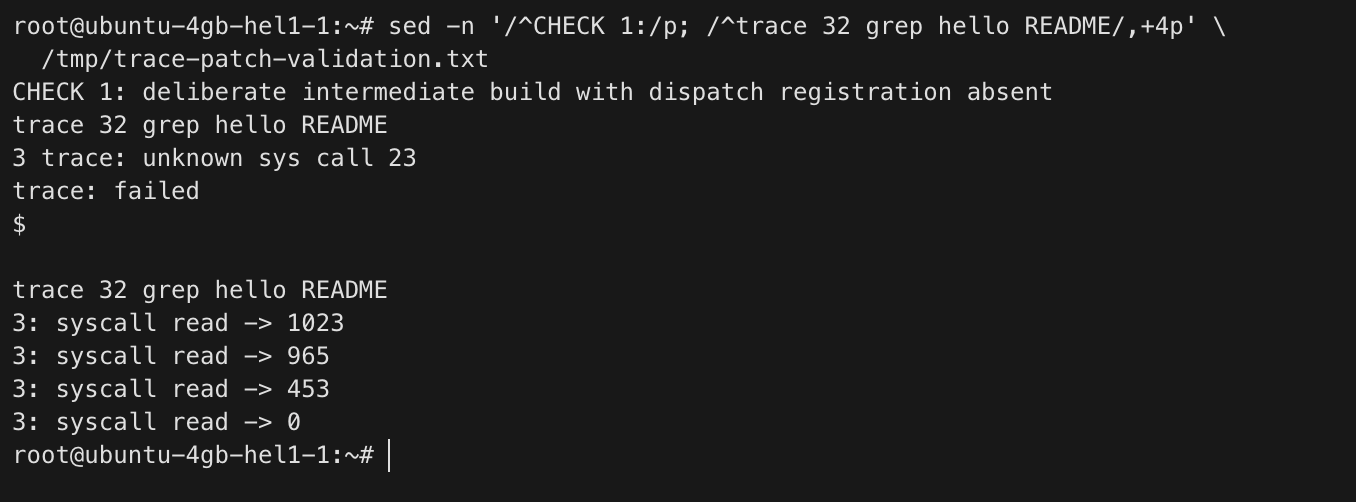
\includegraphics[width=\linewidth,height=0.67\textheight,keepaspectratio]{Lab9-10/evidence/screenshots/lab10-check1-terminal.png}
\end{minipage}\par\medskip

The test then restored the dispatch entry and rebuilt. Read, open and
close masks worked, and
{\ttfamily\fontsize{10}{12}\selectfont trace 2 usertests forkforkfork}
ended with {\ttfamily\fontsize{10}{12}\selectfont ALL TESTS PASSED}. The
test verifies that the mask field belongs inside
{\ttfamily\fontsize{10}{12}\selectfont struct proc} through a successful
kernel build, and exercises inheritance through real child processes.
The complete build and boot record is
{\ttfamily\fontsize{10}{12}\selectfont evidence/tra\allowbreak{}ce-patch-val\allowbreak{}idation.txt}.
The reproducible checker is
{\ttfamily\fontsize{10}{12}\selectfont scripts/chec\allowbreak{}k-trace-patc\allowbreak{}h.py};
use it only with a clean disposable checkout because it applies the
patch and rebuilds the generated disk.

\subsection{Lab 10 Reporting the completed
call}\label{lab-10-reporting-the-completed-call}

The dispatcher first executes
{\ttfamily\fontsize{10}{12}\selectfont syscalls[num\allowbreak{}]()} and
stores the result in the saved a0 register. It then tests the selected
bit and prints the PID, a human-readable name, and the return value
through printk. Printing after the call is essential: printing before
dispatch would observe the argument or old register contents rather than
the completed return value. The name array uses designated initializers
corresponding to the header constants, rather than relying on an assumed
contiguous textual order.

The condition also checks that num is below 32 before shifting a 32-bit
mask. The implemented call numbers are below that limit. This protects
the shift operation but does not turn the lab into a general tracer for
arbitrary larger syscall-number spaces. Calls that never return, such as
exit, do not pass through this post-return print site. The report
therefore does not claim that the all-bits mask must print a line for
every possible process event.

For mask 32, bit five selects SYS\_read. The observed command produced:

\par\noindent\begin{minipage}{\linewidth}

\begin{lstlisting}
$ trace 32 grep hello README
95: syscall read -> 1023
95: syscall read -> 965
95: syscall read -> 453
95: syscall read -> 0
\end{lstlisting}

\end{minipage}\par

The three positive results sum to 2441, the README's length in this
image, followed by a zero-length read at EOF. PID values identify this
run and may change with the number of preceding shell commands. The mask
explains the absence of open and close lines; it does not mean grep
stopped using those calls.

\subsection{Lab 10 Masks that expose different
behavior}\label{lab-10-masks-that-expose-different-behavior}

An all-bits-positive mask of 2147483647 reported trace itself, exec,
open, the read sequence, and close. Trace can report its own successful
return because the handler installs the mask before the dispatcher's
post-call test. Exec returned 3 here, the argument count used by this
xv6 implementation, rather than the zero that someone might expect from
a different interface.

For write-only tracing, 65536 sets bit sixteen. Echo wrote two bytes for
{\ttfamily\fontsize{10}{12}\selectfont hi} and one for the newline; the
trace message appeared between those operations. For open and close
only, the mask is
{\ttfamily\fontsize{10}{12}\selectfont (1 << 15) | (1 << 21) = 2129920}.
The observed output contains precisely those names:

\par\noindent\begin{minipage}{\linewidth}

\begin{lstlisting}
$ trace 2147483647 grep hello README
96: syscall trace -> 0
96: syscall exec -> 3
96: syscall open -> 3
96: syscall read -> 1023
96: syscall read -> 965
96: syscall read -> 453
96: syscall read -> 0
96: syscall close -> 0
$ trace 65536 echo hi
hi97: syscall write -> 2

97: syscall write -> 1
$ trace 2129920 grep hello README
98: syscall open -> 3
98: syscall close -> 0
\end{lstlisting}

\end{minipage}\par

The fork-only mask is 2, selecting bit one.
{\ttfamily\fontsize{10}{12}\selectfont usertests forkforkfork} created
enough children to reach the process-table limit, so a return value of
minus one was expected at saturation. Multiple PIDs printing lines
demonstrate the inherited mask rather than one parent printing all
events. The final test result was:

\par\noindent\begin{minipage}{\linewidth}

\begin{lstlisting}
102: syscall fork -> 148
103: syscall fork -> 156
103: syscall fork -> 157
103: syscall fork -> 158
103: syscall fork -> 159
103: syscall fork -> 160
103: syscall fork -> -1
OK
ALL TESTS PASSED
$ echo tracing-off
tracing-off
$
\end{lstlisting}

\end{minipage}\par

The subsequent ordinary
{\ttfamily\fontsize{10}{12}\selectfont echo tracing-off} produced its
text without a syscall trace. This checks the independent-process case
as well as inheritance. The test runner fails if the distinctive read,
write, open, saturation, and success markers are absent, and retains the
whole console stream rather than only the final success line.

\subsection{Limits and conclusion}\label{limits-and-conclusion}

The Linux and xv6 observations demonstrate two ways to inspect a
system-call interface. The Linux trace includes loader and library work
outside the explicit C statements. The xv6 facility instead sits
directly in the teaching kernel's dispatcher and is intentionally
limited to a per-process bit mask, a name, and a return value. It does
not decode pointers or copy user buffers like a general strace
implementation.

The additional native L9 screenshots use direct terminal stdout: the
program emits three writes of 27, 20 and 33 bytes (80 in total), whereas
the earlier piped recording combined them into one buffered write. The
six calls on fd 3 are unchanged. The first fixed-length sed excerpt
interleaved stdout writes; the second capture filters these out and
shows the complete six-call file sequence.

\subsection{Execution captures and code
excerpts}\label{execution-captures-and-code-excerpts}

Native Terminal screenshots: L9 and final L10 were run live; the two
labeled audit figures show saved verification output.

\par

\medskip\noindent

\begin{minipage}{\linewidth}\setstretch{1.0}
\captionof*{figure}{Figura 2. Native Linux strace: six file calls, ls stdout and openat summary}
\centering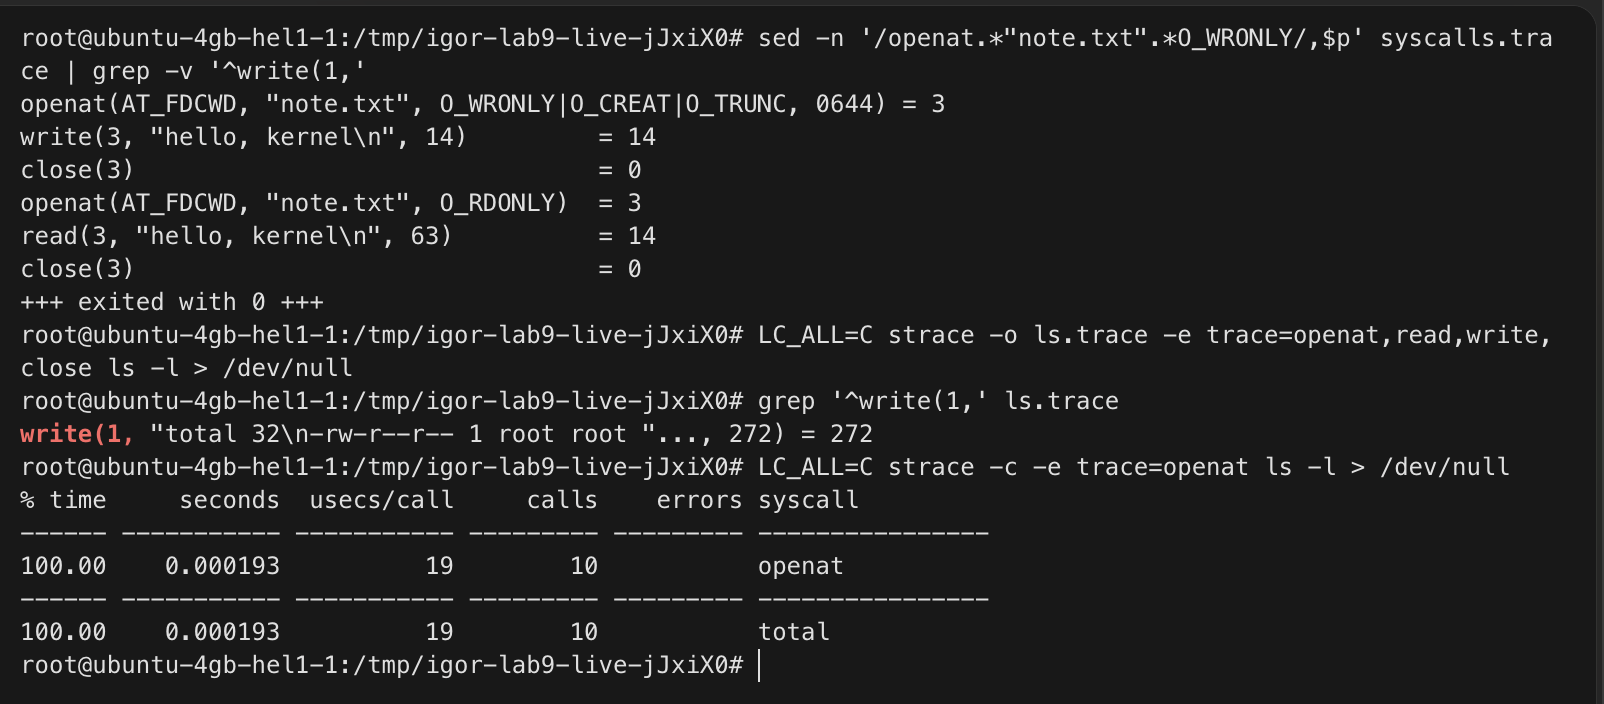
\includegraphics[width=\linewidth,height=0.67\textheight,keepaspectratio]{Lab9-10/evidence/screenshots/lab9-file-calls-terminal.png}
\end{minipage}\par\medskip

\par

\medskip\noindent

\begin{minipage}{\linewidth}\setstretch{1.0}
\captionof*{figure}{Figura 3. Native Linux strace: direct-terminal stdout writes}
\centering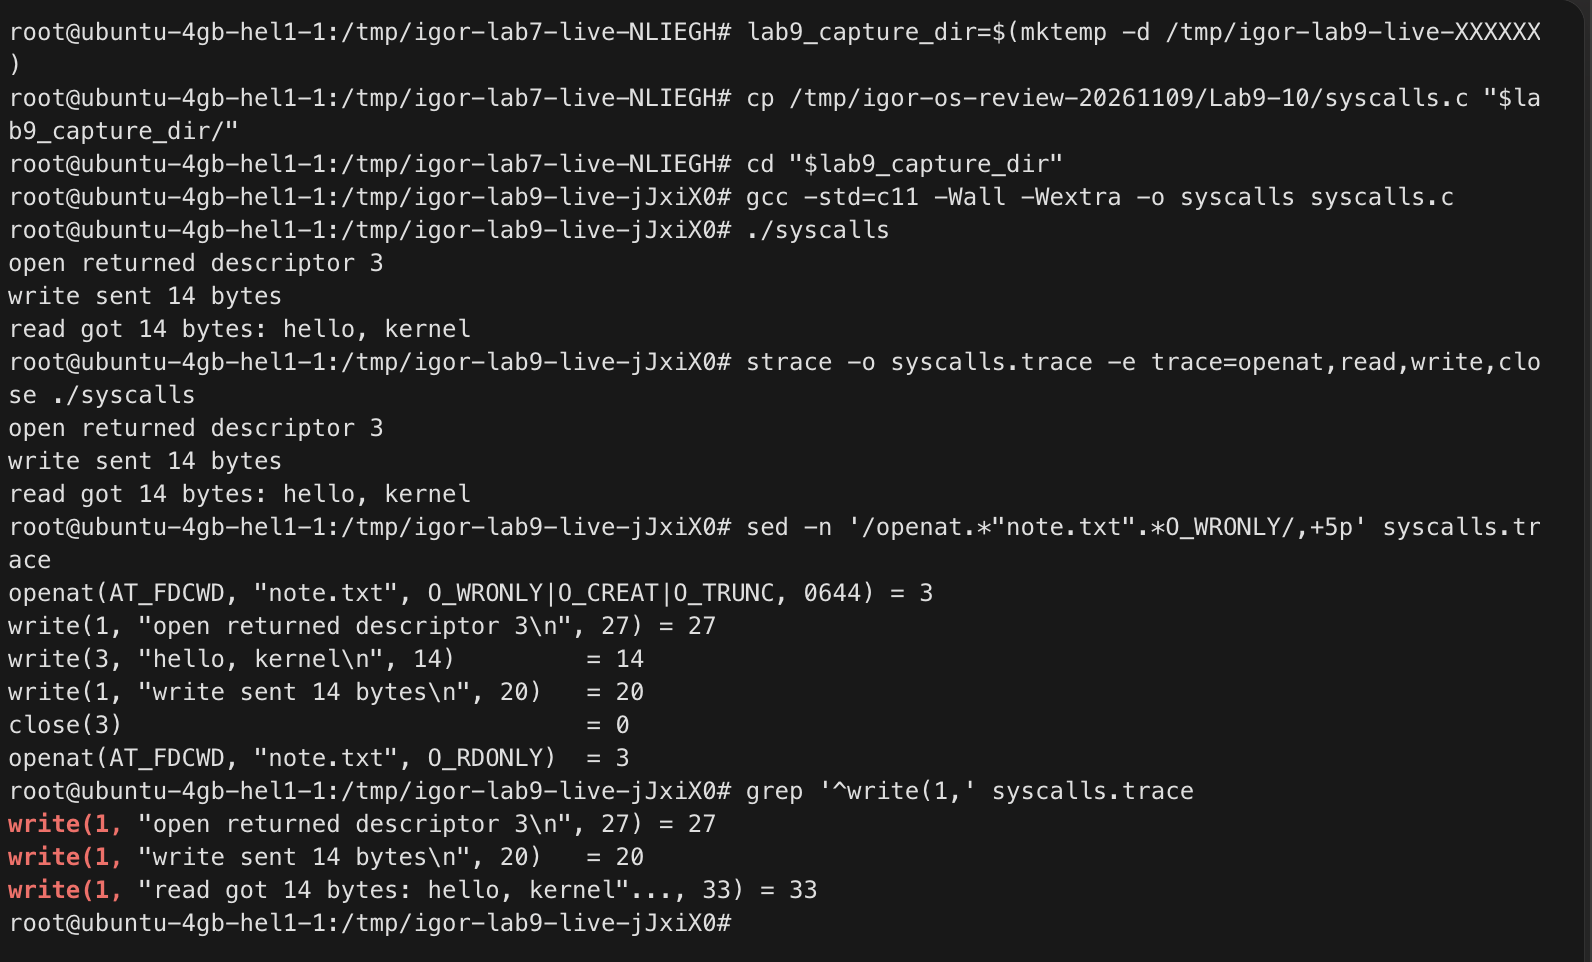
\includegraphics[width=\linewidth,height=0.67\textheight,keepaspectratio]{Lab9-10/evidence/screenshots/lab9-stdout-terminal.png}
\end{minipage}\par\medskip

\par

\medskip\noindent

\begin{minipage}{\linewidth}\setstretch{1.0}
\captionof*{figure}{Figura 4. Native xv6 execution: read, all-call, open/close and write masks}
\centering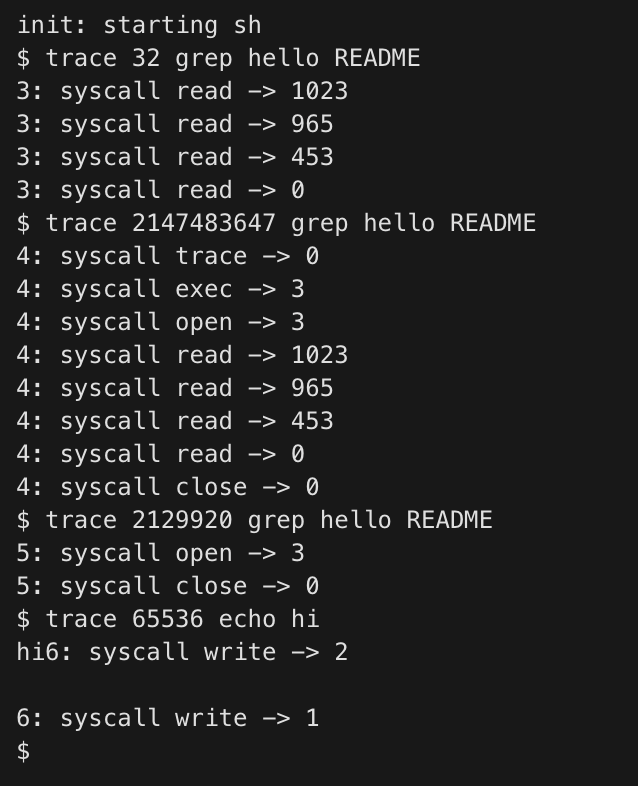
\includegraphics[width=\linewidth,height=0.67\textheight,keepaspectratio]{Lab9-10/evidence/screenshots/lab10-masks-terminal.png}
\end{minipage}\par\medskip

\par

\medskip\noindent

\begin{minipage}{\linewidth}\setstretch{1.0}
\captionof*{figure}{Figura 5. Native xv6 execution: fork test command and inherited tracing}
\centering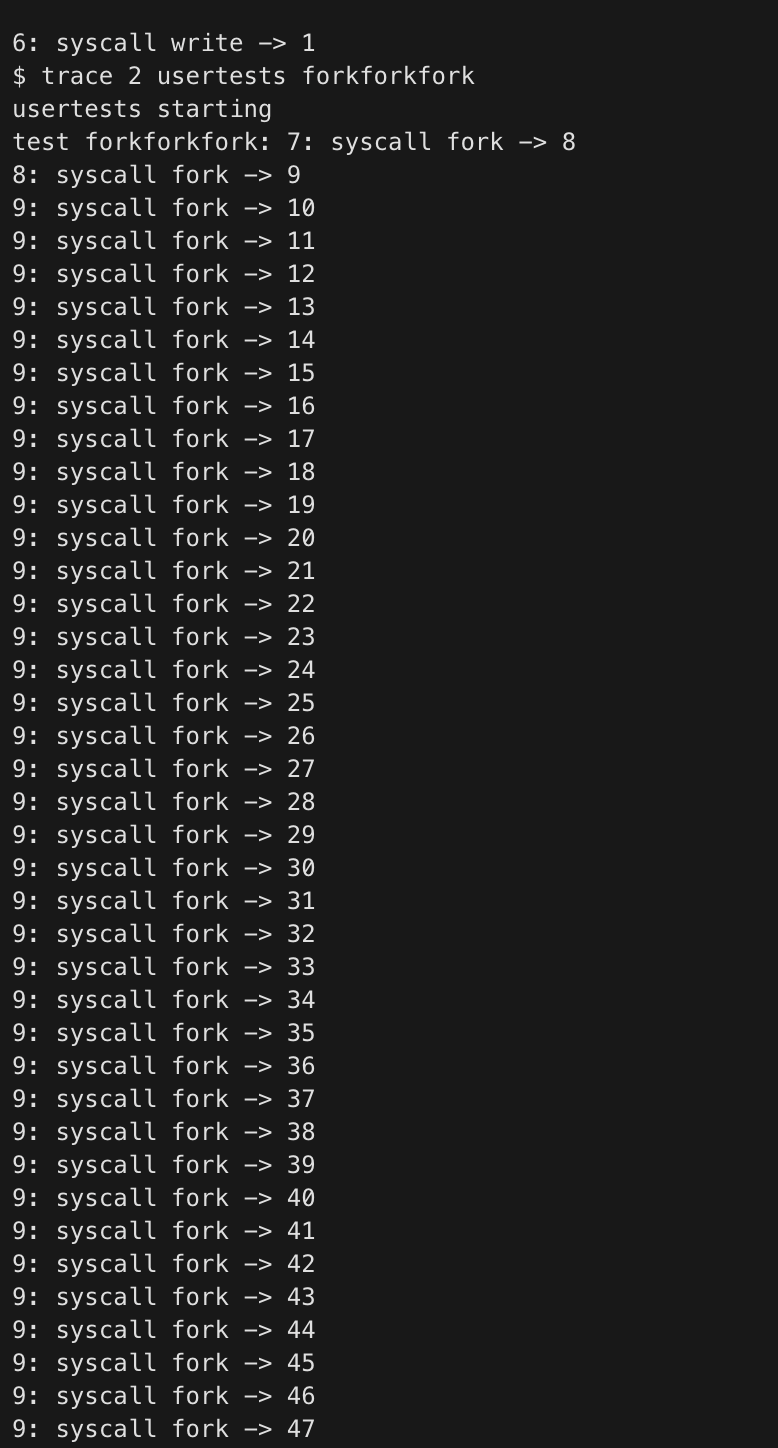
\includegraphics[width=\linewidth,height=0.67\textheight,keepaspectratio]{Lab9-10/evidence/screenshots/lab10-fork-start-terminal.png}
\end{minipage}\par\medskip

\par

\medskip\noindent

\begin{minipage}{\linewidth}\setstretch{1.0}
\captionof*{figure}{Figura 6. Native xv6 execution: fork test completion and ALL TESTS PASSED}
\centering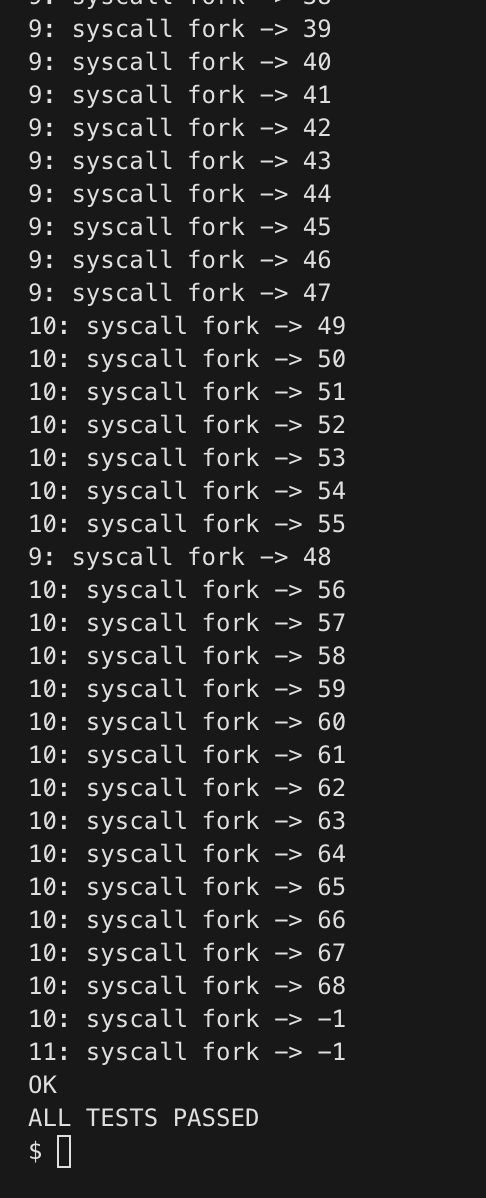
\includegraphics[width=\linewidth,height=0.67\textheight,keepaspectratio]{Lab9-10/evidence/screenshots/lab10-fork-pass-terminal.png}
\end{minipage}\par\medskip

\par

\medskip\noindent

\begin{minipage}{\linewidth}\setstretch{1.0}
\captionof*{figure}{Figura 7. Native Terminal screenshot of the saved audit record: verified MIT base, patch application checks, and passing fork inheritance test. The head and tail commands display the beginning and end of the complete committed log.}
\centering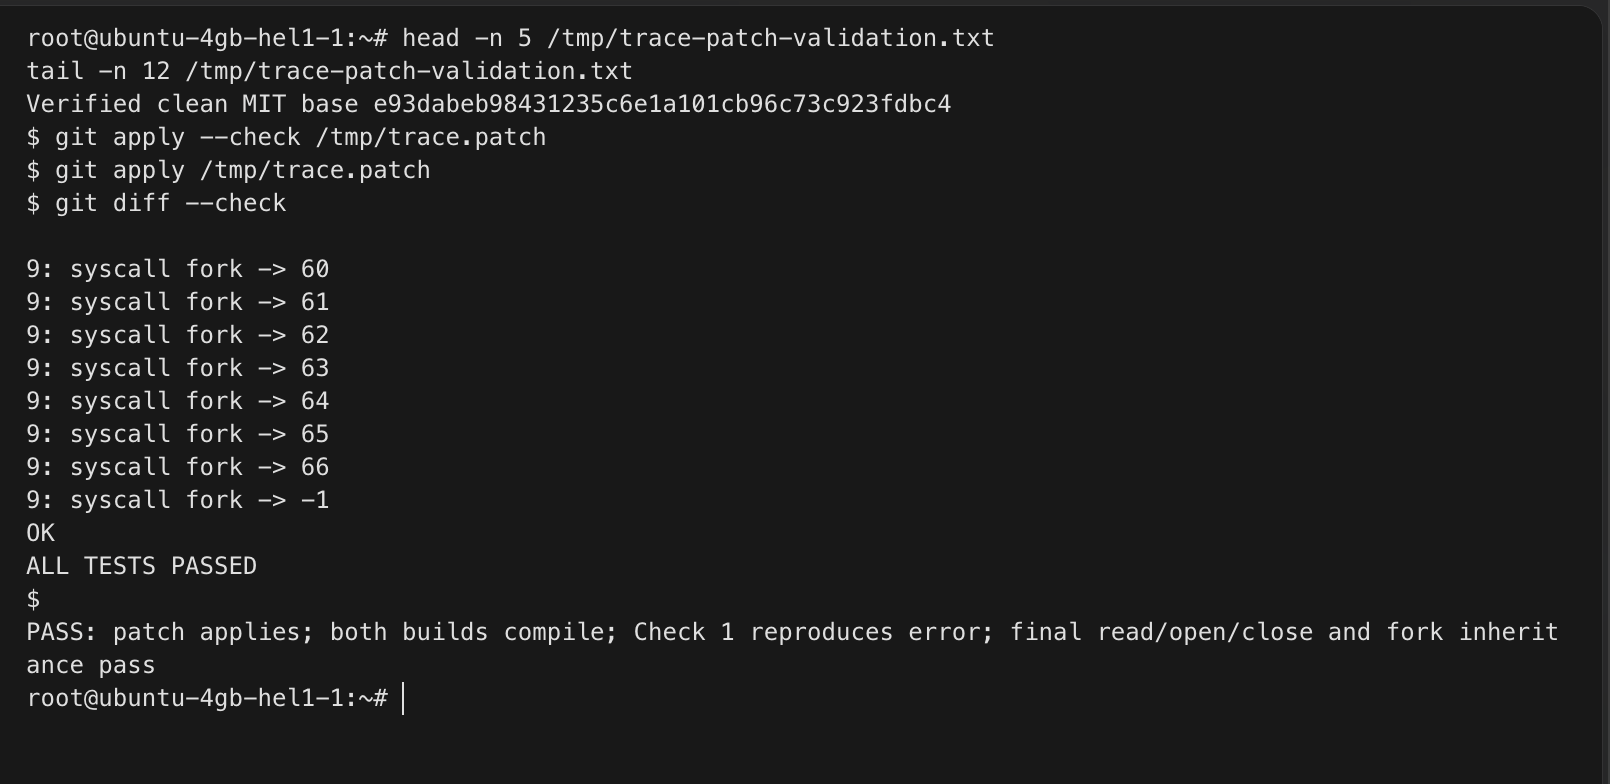
\includegraphics[width=\linewidth,height=0.67\textheight,keepaspectratio]{Lab9-10/evidence/screenshots/lab10-patch-pass-terminal.png}
\end{minipage}\par\medskip

\subsection{Source excerpts from the submitted
implementation}\label{source-excerpts-from-the-submitted-implementation}

\subsubsection{Linux file operations}\label{linux-file-operations}

\begin{lstlisting}[language=C]
/* Lab 9: observe open, write, read, and close with strace. */
#include <fcntl.h>
#include <stdio.h>
#include <string.h>
#include <unistd.h>

int main(void)
{
    const char *msg = "hello, kernel\n";
    int fd = open("note.txt", O_CREAT | O_WRONLY | O_TRUNC, 0644);
    if (fd < 0) {
        perror("open for writing");
        return 1;
    }

    printf("open returned descriptor %d\n", fd);
    ssize_t n = write(fd, msg, strlen(msg));
    if (n < 0 || (size_t)n != strlen(msg)) {
        perror("write");
        close(fd);
        return 1;
    }
    printf("write sent %zd bytes\n", n);
    if (close(fd) < 0) {
        perror("close after writing");
        return 1;
    }

    fd = open("note.txt", O_RDONLY);
    if (fd < 0) {
        perror("open for reading");
        return 1;
    }
    char buf[64];
    n = read(fd, buf, sizeof(buf) - 1);
    if (n < 0) {
        perror("read");
        close(fd);
        return 1;
    }
    buf[n] = '\0';
    printf("read got %zd bytes: %s", n, buf);
    if (close(fd) < 0) {
        perror("close after reading");
        return 1;
    }
    return 0;
}
\end{lstlisting}

\subsubsection{xv6 user utility}\label{xv6-user-utility}

\par\noindent\begin{minipage}{\linewidth}

\begin{lstlisting}[language=C]
#include "kernel/types.h"
#include "kernel/stat.h"
#include "user/user.h"

int
main(int argc, char *argv[])
{
  if (argc < 3) {
    fprintf(2, "usage: trace mask command [args...]\n");
    exit(1);
  }
  if (trace(atoi(argv[1])) < 0) {
    fprintf(2, "trace: failed\n");
    exit(1);
  }
  exec(argv[2], argv + 2);
  fprintf(2, "trace: exec %s failed\n", argv[2]);
  exit(1);
}
\end{lstlisting}

\end{minipage}\par

\subsubsection{Kernel handler}\label{kernel-handler}

\par\noindent\begin{minipage}{\linewidth}

\begin{lstlisting}[language=C]
uint64
sys_trace(void)
{
  int mask;
  argint(0, &mask);
  myproc()->trace_mask = mask;
  return 0;
}
\end{lstlisting}

\end{minipage}\par

\subsubsection{Dispatch after the system call
returns}\label{dispatch-after-the-system-call-returns}

\par\noindent\begin{minipage}{\linewidth}

\begin{lstlisting}[language=C]
void
syscall(void)
{
  int num;
  struct proc *p = myproc();

  num = p->trapframe->a7;
  if (num > 0 && num < NELEM(syscalls) && syscalls[num]) {
    // Use num to lookup the system call function for num, call it,
    // and store its return value in p->trapframe->a0
    p->trapframe->a0 = syscalls[num]();
    if (num < 32 && (p->trace_mask & (1U << num)))
      printk("%d: syscall %s -> %ld\n", p->pid, syscallnames[num], p->trapframe->a0);
  } else {
    printk("%d %s: unknown sys call %d\n", p->pid, p->name, num);
    p->trapframe->a0 = -1;
  }
}
\end{lstlisting}

\end{minipage}\par

\subsubsection{Per-process state, initialization and
inheritance}\label{per-process-state-initialization-and-inheritance}

These are excerpts from kernel/proc.h and kernel/proc.c respectively;
the complete context is in the buildable tree and the validated patch.

\begin{lstlisting}[language=C]
  struct file *ofile[NOFILE];  // Open files
  struct inode *cwd;           // Current directory
  char name[16];               // Process name (debugging)
  int trace_mask;              // System calls selected for tracing
};


found:
  p->pid = allocpid();
  p->state = USED;
  p->trace_mask = 0;

  // Allocate a trapframe page.
  if ((p->trapframe = (struct trapframe *)kalloc()) == 0) {

    if (p->ofile[i])
      np->ofile[i] = filedup(p->ofile[i]);
  np->cwd = idup(p->cwd);

  safestrcpy(np->name, p->name, sizeof(p->name));
  np->trace_mask = p->trace_mask;

  pid = np->pid;
\end{lstlisting}

\par\noindent\begin{minipage}{\linewidth}

\section{Concluzie}\label{concluzie}

Înregistrările strace separă operațiile pe fișier de afișarea
diagnosticului și de efectele buffering-ului. Implementarea trace și
validarea pe baza xv6 declarată fac traseul apelului și efectul măștilor
verificabile prin cod, patch și execuție.

\end{minipage}\par

\end{document}
